\documentclass[../thesis.tex]{subfiles}
\begin{document}
\chapter{Twitter Sentiment Results}
\label{ch:sentimentresults}

We find each of our different Twitter sentiment strategies have overall strong results. Different models have differing effects on various stocks. For all of our models, 100\% beat the baseline for all stocks with baseline \textit{buy-and-hold} losses. This unanimous success for poor performing stocks gives great promise towards a live-trading implementation during poor overall stock market performances. Stocks that have a strong baseline performances are rarely beaten by any of our strategies, but still mostly generate positive profits within roughly 10\% of the strong baseline measure. Although, each specific model utilizing the extended feature sentiment finds at least two stocks with performances that beat the baseline by over 50\%. On an individual stock level, our results have somewhat random performances on each model for different stocks. This lack of consistency is due to the difference in data and sentiment for each stock. Because we fit the model for each stock on each machine learning algorithm, it would be highly improbable to see one model give persistent and consistent results due to the random nature of market movement. 

Of the 16 stocks we tested, we examine 8 in-depth that have the most remarkable results across different algorithms. However, we do discuss the overall results using all of the stocks that we tested at the end of this chapter. We exclude the lowest performing in our in-depth discussion of the models to emphasize the highest performing stocks for our strategies. Common practice in the field is to focus on and examine the highest performing stocks across different strategies \cite{Aldridge2010}. Therefore, we choose \texttt{DIS, EBAY, SBUX, BIG, NKE, AMD, COLM, and MNST}. Most of these stocks share a common feature: the baseline strategy posts sizable losses, whereas our trading algorithms make profit when the stock does poorly. Therefore, stocks that had strong baseline performances during the trading period such as \texttt{HAS} or \texttt{FB}, were excluded from individual analysis of each of the models and are instead examined in Figure~\ref{alltweetresults}. 

As a whole, it would be difficult to trade using this entire group of tested stocks, but our testing reveals some encouraging results. Trading on this Twitter sentiment strategy certainly comes with lots of risk and is at an individuals discretion. However, individual results that beat the baseline by nearly 80 or more percentage points offer some starting points for making a live trading implementation. Specifically, using our deep learning strategy on \texttt{SBUX} nets a 54.5\% profit over the trading period, while the baseline \textit{buy-and-hold} nets a loss of 23.7\%. The stacking lenient strategy for \texttt{MNST} nets a 50\% profit while the baseline nets a loss of 31.2\%. Another encouraging result worth pursuing in live trading is the extended model decision tree algorithm for \texttt{AMD}. For this particular stock, our algorithm nets a 529.1\% profit, more than doubling the baseline's already impressive 207.3\% profit. Our research shows that starting with these three stocks and the associated strategies would be a great start to a sample portfolio.

\section{Simplistic Model}
Our simplistic model has the worst performance of any of the tested strategies. Only a few of the stocks tested had truly notable performances. Figure~\ref{simpleresults} shows the performance of a selection of stocks that were tested. We rarely find any machine learning algorithm actually beat the baseline. Only 29.4\% of stocks tested ended up beating the baseline. The vast majority of stocks tested performed like \texttt{COLM}, with all four of our machine learning algorithms generating profits slightly below or right at the baseline. However, some did actually find success. \texttt{MNST}'s MLP beat the baseline by 31.2\% whereas \texttt{SBUX}'s decision tree classifier beat the baseline by 50.7\%. Only a minority of stocks show profitable trading margins. We need to utilize a more advanced feature set to more effectively predict following day stock price movement. We find improvement across the board by adding more inputs into the model as seen in the following section. 

\begin{figure}[h]
\centering
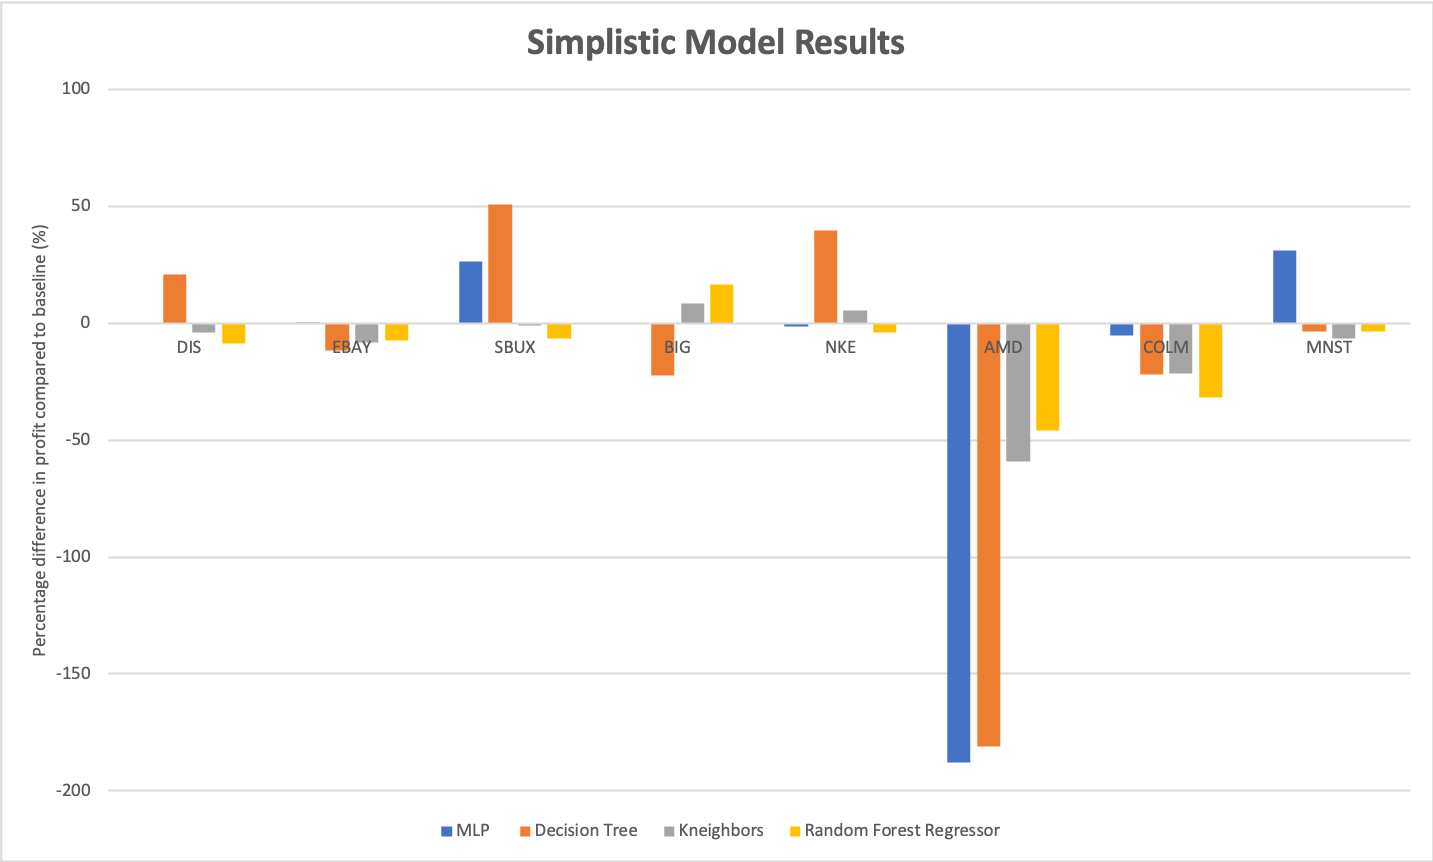
\includegraphics[width=.9\textwidth]{BasicModelResults.png}
\caption{Simplistic Model Results \label{overflow}}
\label{simpleresults}
\end{figure}

\section{Extended Model}
By adding total tweets, retweets, and favorites as additional features, we see an overall improvement over the simplistic model that only uses closing price and twitter sentiment. Figure~\ref{complexresults} shows the performance of a selection of stocks that were tested. We find that 82.4\% of the stocks tested have a particular algorithm that beats the baseline. This is an improvement of 53\% moving to a model with more features. This means that including features such as amount of tweets and retweets are useful for stock trading. Specifically, \texttt{AMD} has the most remarkable performance, with the decision tree classifier generating 529.1\% profit and more than doubling the baseline profit. We find \texttt{MNST} to also have impressive returns with this model. The decision tree classifier generates a 79\% profit while the baseline nets a loss of 31.2\%. The random forest regressor of \texttt{BIG} generates 88.7\% profit, beating the baseline by 55.7\%. These returns for specific models on specific stocks are significant enough to implement for a realtime for-profit trading algorithm, showing that Twitter sentiment can be used to aid stock trading. 

\begin{figure}[h]
\centering
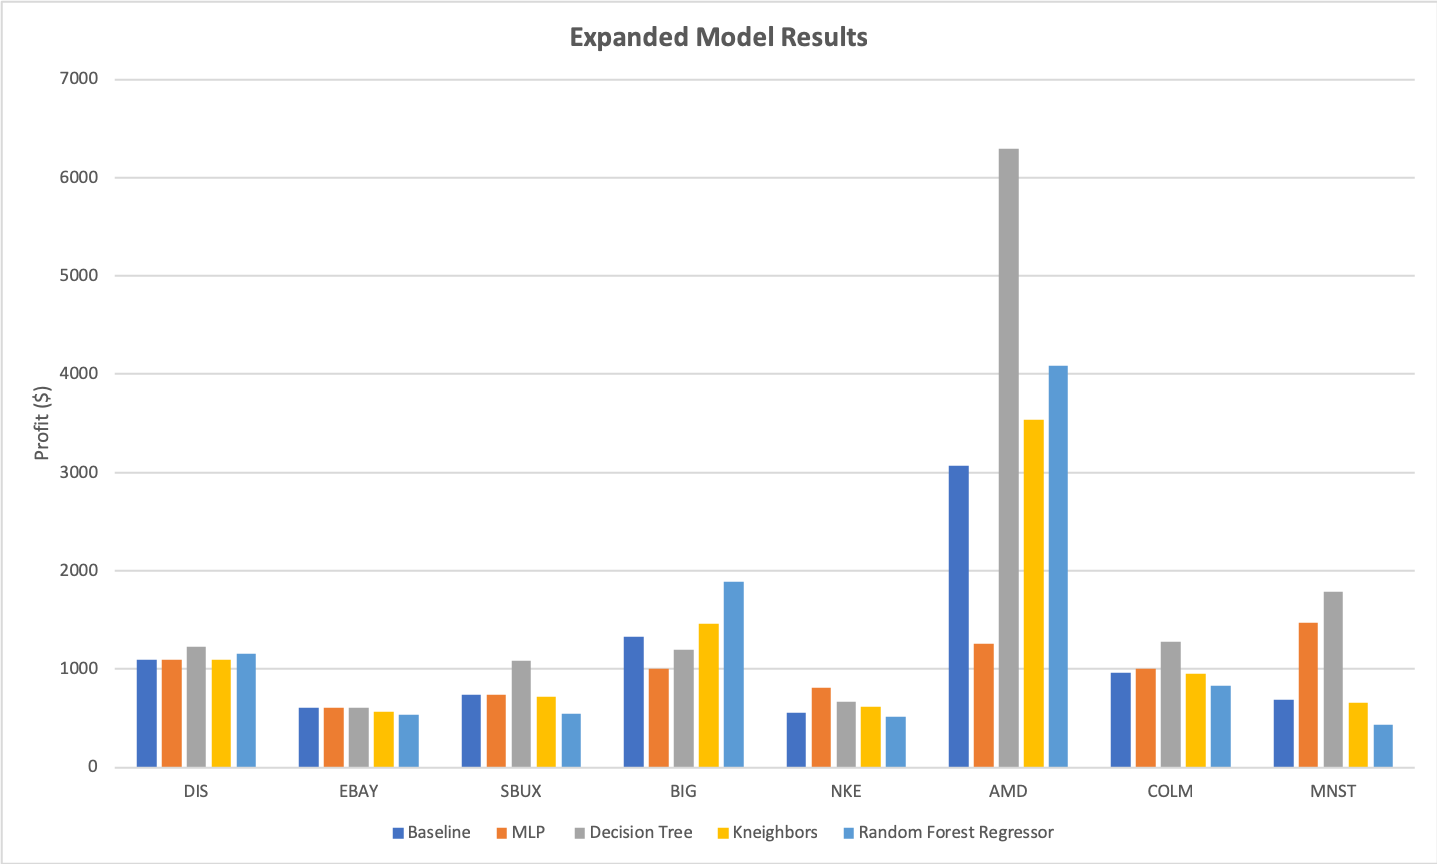
\includegraphics[width=.9\textwidth]{ComplexModelResults.png}
\caption{Extended Model Results \label{overflow}}
\label{complexresults}
\end{figure}

\section{Stacking Model}
Our stacking model that aggregates all of our various machine learning models into one buy or sell signal doesn't perform as well as the extended model, but handily beats the basic model. Figure~\ref{complexresults} shows the performance of a selection of stocks that were tested. We find that 58.8\% of the stocks using the conservative strategy beat the baseline, while only 29.4\% of the lenient strategy beat the baseline. These results show how the conservative strategy performs far more consistently than the lenient strategy. \texttt{EBAY's} conservative strategy has a 6.9\% return while the baseline has a 39.5\% loss. \texttt{MNST} nets a 50\% profit while the baseline records a loss of 31.2\% while using the lenient strategy. This performance sets a high individual performance threshold for this model, as the baseline measure is significantly negative while our strategy has large positive returns. In these results, the stocks that end up beating the baseline are correlated with baseline losses over the trading period. While a few stocks do end up beating a high performing baseline, this strategy like others using Twitter sentiment, performs much better when the stock does poorly over the trading period. 

\begin{figure}[h]
\centering
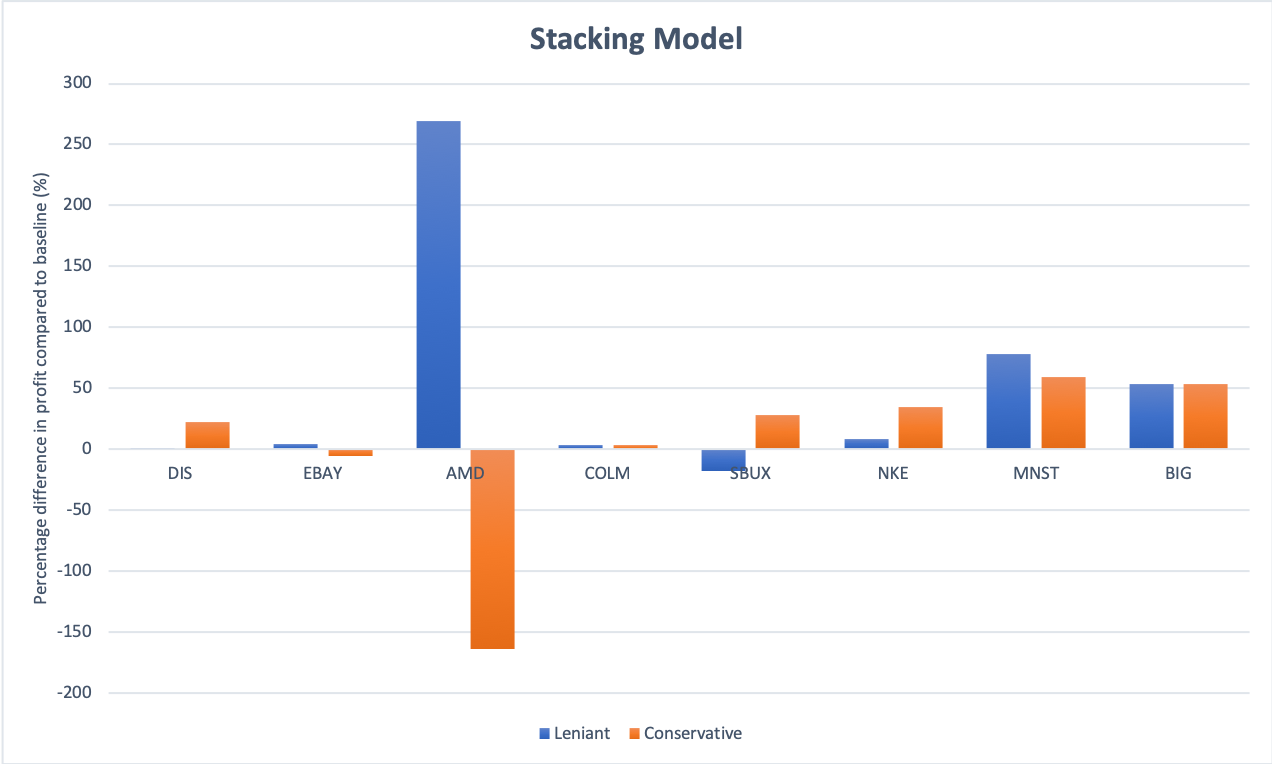
\includegraphics[width=.9\textwidth]{BoostingModelResults.png}
\caption{Stacking Model Results \label{overflow}}
\label{stackingresults}
\end{figure}

\section{Deep Learning Model}
Our deep learning model acts differently than any of the above models, as it predicts the price of the following days close. This model has more average performance, but is far more consistent. Rarely does a particular stock trading on the strategy fall significantly below the baseline. Figure~\ref{deepresults} shows our results for some specific stocks within the data. \texttt{DIS, NKE,} and \texttt{COLM} categorize the results of this model well -- showing how the strategy hovers close to the baseline and gives consistent performance. Interestingly, \texttt{EBAY} and \texttt{SBUX}, perform far better than the baseline. There is a respective improvement of \$559.53 and \$785.71 for our strategy over the baseline. 


For this model we don't find as many instances of beating the baseline as some of our other models. This is most likely attributed to the accuracy of the predicted stock prices. The RMSE of all of our stocks range between 1.5 and 2.5, signifying that our model is able to predict the closing price of stocks extremely closely. While the predicted price is close, it isn't accurate enough to be consistently profitable. This performance is most likely due the model predicting stock prices for multiple days in a row either above or below the current price. This prediction differs from the other models that all predict price signal changes. We find that this change in prediction hampers performance for our end-of-day trading strategy that is entirely reliant on price signal changes. Future work could predict multiple days of stock prices in the future and then act on sustained performance rather than specific day-by-day changes to help with this issue in our strategy. 

\begin{figure}[h]
\centering
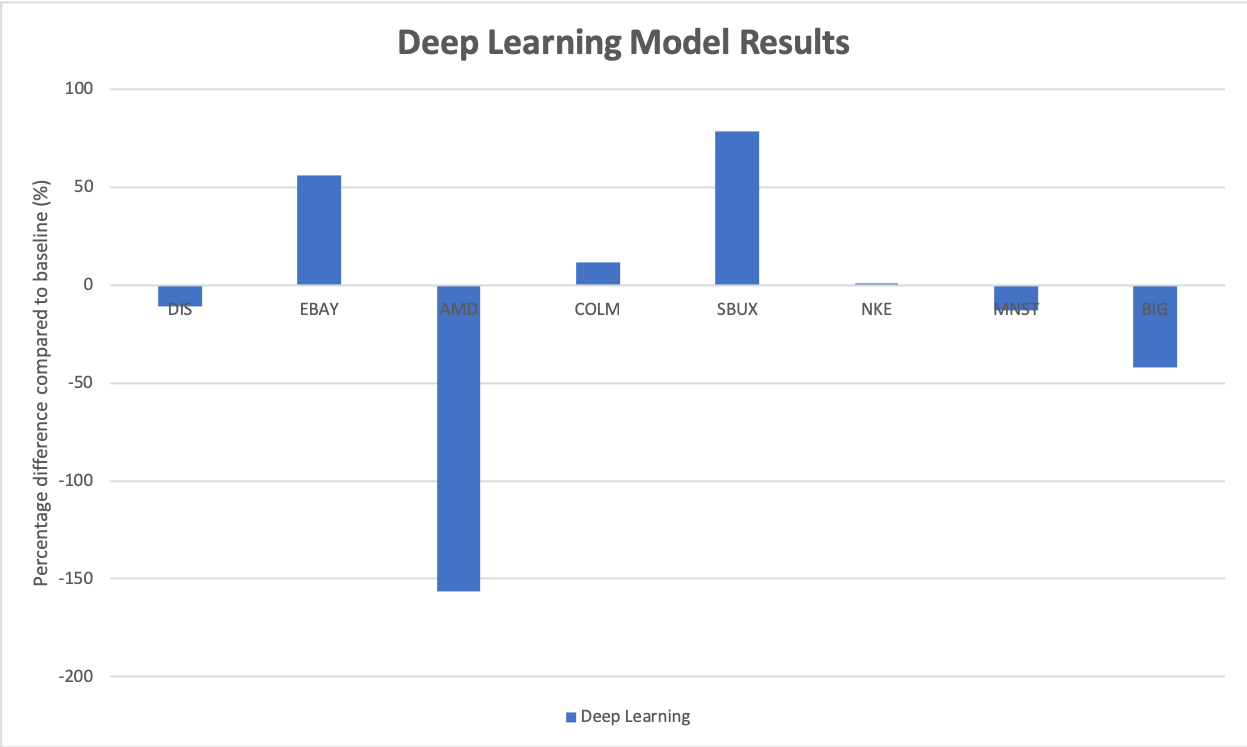
\includegraphics[width=.9\textwidth]{DeepLearningResults.png}
\caption{Deep Learning Model Results \label{overflow}}
\label{deepresults}
\end{figure}

\section{Discussion and Comparison}

Now that we have examined some particular notable performances of specific models, we must identify trends between all of our models. Figure~\ref{alltweetresults} shows our results for all 16 stocks tested. We don't find that one model has particularly astounding performance across all of the stocks tested. However, the decision tree classifier is the most successful of the models examined. With a median score of 6.4\% and an upper quartile score of 28.7\%, this classifier has the most positive results as it has the largest concentration of the models with performances that beat the baseline. Both of our strategies that use the stacking model have positive medians, signaling its effectiveness. We additionally find that the upper quartile performances for each model are all greater than the baseline. Excepting the decision tree classifier and conservative stacking model, we see a consistent spread between the upper and lower quartiles of roughly 25 percentage points. As discussed in the above sections, each of our strategies has a few stocks that generate incredible performance. This performance is reflected in Figure~\ref{alltweetresults} as we see a collection of positive outlier datapoints above each different model. 

However, we also find some limitations with our models and data. Even though the 16 stocks we examined for our sentiment strategies were spread across different industries, it is still possible that skew exists within our data. Incorporating many more stocks to test our models would give more basis to our findings. We are looking at a very small subset of the entire market. But, this small subset is a result of data availability and expense. For acquiring Twitter data, Twitter makes data available at a fee that is prohibitively expensive. Our method for scraping twitter data is incredibly time intensive and restricts our study to 16 stocks.  A more thorough study would examine a greater collection of stocks. Additionally, examining more classifiers and regressors could lead to discovering more machine learning algorithms that are highly productive. 

\begin{figure}[h]
\centering
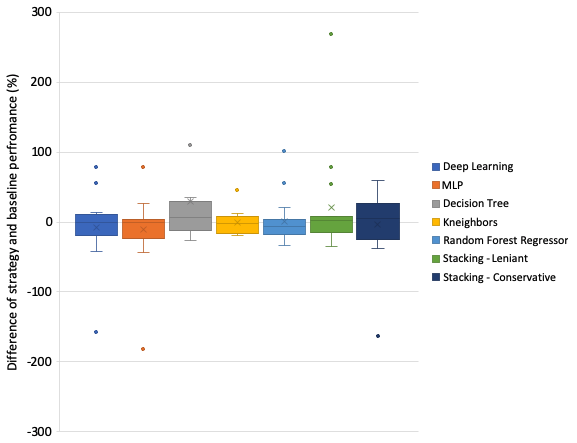
\includegraphics[width=2.2\textwidth]{alltwitterstrategies.png}
\caption{Twitter Sentiment Results Compared \label{overflow}}
\label{alltweetresults}
\end{figure}

\end{document}
